 % !TEX program = xelatex
\documentclass{article}
\usepackage[margin=1in]{geometry}
\usepackage{amsmath,amsthm}
\usepackage{amsfonts}
\usepackage{graphicx}
\usepackage{xcolor}
\usepackage{ulem}
\usepackage{wrapfig}
\usepackage{booktabs}
\usepackage{comment}
\DeclareMathOperator{\tr}{tr}
\DeclareMathOperator{\sign}{sign}
% Calligraphic fonts
\newcommand{\calA}{{\cal A}}
\newcommand{\calB}{{\cal B}}
\newcommand{\calC}{{\cal C}}
\newcommand{\calD}{{\cal D}}
\newcommand{\calE}{{\cal E}}
\newcommand{\calF}{{\cal F}}
\newcommand{\calG}{{\cal G}}
\newcommand{\calH}{{\cal H}}
\newcommand{\calI}{{\cal I}}
\newcommand{\calJ}{{\cal J}}
\newcommand{\calK}{{\cal K}}
\newcommand{\calL}{{\cal L}}
\newcommand{\calM}{{\cal M}}
\newcommand{\calN}{{\cal N}}
\newcommand{\calO}{{\cal O}}
\newcommand{\calP}{{\cal P}}
\newcommand{\calQ}{{\cal Q}}
\newcommand{\calR}{{\cal R}}
\newcommand{\calS}{{\cal S}}
\newcommand{\calT}{{\cal T}}
\newcommand{\calU}{{\cal U}}
\newcommand{\calV}{{\cal V}}
\newcommand{\calW}{{\cal W}}
\newcommand{\calX}{{\cal X}}
\newcommand{\calY}{{\cal Y}}
\newcommand{\calZ}{{\cal Z}}

% Sets:
\newcommand{\setA}{\textsf{A}}
\newcommand{\setB}{\textsf{B}}
\newcommand{\setC}{\textsf{C}}
\newcommand{\setD}{\textsf{D}}
\newcommand{\setE}{\textsf{E}}
\newcommand{\setF}{\textsf{F}}
\newcommand{\setG}{\textsf{G}}
\newcommand{\setH}{\textsf{H}}
\newcommand{\setI}{\textsf{I}}
\newcommand{\setJ}{\textsf{J}}
\newcommand{\setK}{\textsf{K}}
\newcommand{\setL}{\textsf{L}}
\newcommand{\setM}{\textsf{M}}
\newcommand{\setN}{\textsf{N}}
\newcommand{\setO}{\textsf{O}}
\newcommand{\setP}{\textsf{P}}
\newcommand{\setQ}{\textsf{Q}}
\newcommand{\setR}{\textsf{R}}
\newcommand{\setS}{\textsf{S}}
\newcommand{\setT}{\textsf{T}}
\newcommand{\setU}{\textsf{U}}
\newcommand{\setV}{\textsf{V}}
\newcommand{\setW}{\textsf{W}}
\newcommand{\setX}{\textsf{X}}
\newcommand{\setY}{\textsf{Y}}
\newcommand{\setZ}{\textsf{Z}}

% Vectors
\newcommand{\bfa}{\mathbf{a}}
\newcommand{\bfb}{\mathbf{b}}
\newcommand{\bfc}{\mathbf{c}}
\newcommand{\bfd}{\mathbf{d}}
\newcommand{\bfe}{\mathbf{e}}
\newcommand{\bff}{\mathbf{f}}
\newcommand{\bfg}{\mathbf{g}}
\newcommand{\bfh}{\mathbf{h}}
\newcommand{\bfi}{\mathbf{i}}
\newcommand{\bfj}{\mathbf{j}}
\newcommand{\bfk}{\mathbf{k}}
\newcommand{\bfl}{\mathbf{l}}
\newcommand{\bfm}{\mathbf{m}}
\newcommand{\bfn}{\mathbf{n}}
\newcommand{\bfo}{\mathbf{o}}
\newcommand{\bfp}{\mathbf{p}}
\newcommand{\bfq}{\mathbf{q}}
\newcommand{\bfr}{\mathbf{r}}
\newcommand{\bfs}{\mathbf{s}}
\newcommand{\bft}{\mathbf{t}}
\newcommand{\bfu}{\mathbf{u}}
\newcommand{\bfv}{\mathbf{v}}
\newcommand{\bfw}{\mathbf{w}}
\newcommand{\bfx}{\mathbf{x}}
\newcommand{\bfy}{\mathbf{y}}
\newcommand{\bfz}{\mathbf{z}}


\newcommand{\bfalpha}{\boldsymbol{\alpha}}
\newcommand{\bfbeta}{\boldsymbol{\beta}}
\newcommand{\bfgamma}{\boldsymbol{\gamma}}
\newcommand{\bfdelta}{\boldsymbol{\delta}}
\newcommand{\bfepsilon}{\boldsymbol{\epsilon}}
\newcommand{\bfzeta}{\boldsymbol{\zeta}}
\newcommand{\bfeta}{\boldsymbol{\eta}}
\newcommand{\bftheta}{\boldsymbol{\theta}}
\newcommand{\bfiota}{\boldsymbol{\iota}}
\newcommand{\bfkappa}{\boldsymbol{\kappa}}
\newcommand{\bflambda}{\boldsymbol{\lambda}}
\newcommand{\bfmu}{\boldsymbol{\mu}}
\newcommand{\bfnu}{\boldsymbol{\nu}}
\newcommand{\bfomicron}{\boldsymbol{\omicron}}
\newcommand{\bfpi}{\boldsymbol{\pi}}
\newcommand{\bfrho}{\boldsymbol{\rho}}
\newcommand{\bfsigma}{\boldsymbol{\sigma}}
\newcommand{\bftau}{\boldsymbol{\tau}}
\newcommand{\bfupsilon}{\boldsymbol{\upsilon}}
\newcommand{\bfphi}{\boldsymbol{\phi}}
\newcommand{\bfchi}{\boldsymbol{\chi}}
\newcommand{\bfpsi}{\boldsymbol{\psi}}
\newcommand{\bfomega}{\boldsymbol{\omega}}
\newcommand{\bfxi}{\boldsymbol{\xi}}
\newcommand{\bfell}{\boldsymbol{\ell}}

% Matrices
\newcommand{\bfA}{\mathbf{A}}
\newcommand{\bfB}{\mathbf{B}}
\newcommand{\bfC}{\mathbf{C}}
\newcommand{\bfD}{\mathbf{D}}
\newcommand{\bfE}{\mathbf{E}}
\newcommand{\bfF}{\mathbf{F}}
\newcommand{\bfG}{\mathbf{G}}
\newcommand{\bfH}{\mathbf{H}}
\newcommand{\bfI}{\mathbf{I}}
\newcommand{\bfJ}{\mathbf{J}}
\newcommand{\bfK}{\mathbf{K}}
\newcommand{\bfL}{\mathbf{L}}
\newcommand{\bfM}{\mathbf{M}}
\newcommand{\bfN}{\mathbf{N}}
\newcommand{\bfO}{\mathbf{O}}
\newcommand{\bfP}{\mathbf{P}}
\newcommand{\bfQ}{\mathbf{Q}}
\newcommand{\bfR}{\mathbf{R}}
\newcommand{\bfS}{\mathbf{S}}
\newcommand{\bfT}{\mathbf{T}}
\newcommand{\bfU}{\mathbf{U}}
\newcommand{\bfV}{\mathbf{V}}
\newcommand{\bfW}{\mathbf{W}}
\newcommand{\bfX}{\mathbf{X}}
\newcommand{\bfY}{\mathbf{Y}}
\newcommand{\bfZ}{\mathbf{Z}}


\newcommand{\bfGamma}{\boldsymbol{\Gamma}}
\newcommand{\bfDelta}{\boldsymbol{\Delta}}
\newcommand{\bfTheta}{\boldsymbol{\Theta}}
\newcommand{\bfLambda}{\boldsymbol{\Lambda}}
\newcommand{\bfPi}{\boldsymbol{\Pi}}
\newcommand{\bfSigma}{\boldsymbol{\Sigma}}
\newcommand{\bfUpsilon}{\boldsymbol{\Upsilon}}
\newcommand{\bfPhi}{\boldsymbol{\Phi}}
\newcommand{\bfPsi}{\boldsymbol{\Psi}}
\newcommand{\bfOmega}{\boldsymbol{\Omega}}


% Blackboard Bold:
\newcommand{\bbA}{\mathbb{A}}
\newcommand{\bbB}{\mathbb{B}}
\newcommand{\bbC}{\mathbb{C}}
\newcommand{\bbD}{\mathbb{D}}
\newcommand{\bbE}{\mathbb{E}}
\newcommand{\bbF}{\mathbb{F}}
\newcommand{\bbG}{\mathbb{G}}
\newcommand{\bbH}{\mathbb{H}}
\newcommand{\bbI}{\mathbb{I}}
\newcommand{\bbJ}{\mathbb{J}}
\newcommand{\bbK}{\mathbb{K}}
\newcommand{\bbL}{\mathbb{L}}
\newcommand{\bbM}{\mathbb{M}}
\newcommand{\bbN}{\mathbb{N}}
\newcommand{\bbO}{\mathbb{O}}
\newcommand{\bbP}{\mathbb{P}}
\newcommand{\bbQ}{\mathbb{Q}}
\newcommand{\bbR}{\mathbb{R}}
\newcommand{\bbS}{\mathbb{S}}
\newcommand{\bbT}{\mathbb{T}}
\newcommand{\bbU}{\mathbb{U}}
\newcommand{\bbV}{\mathbb{V}}
\newcommand{\bbW}{\mathbb{W}}
\newcommand{\bbX}{\mathbb{X}}
\newcommand{\bbY}{\mathbb{Y}}
\newcommand{\bbZ}{\mathbb{Z}}






\title{Rick Eason's Practice Problems}
\author{Instructor: Vikas Dhiman; Originally by: Rick Eason}

\newtheorem{prob}{Problem}
\numberwithin{prob}{section}
\newif\ifsol
\soltrue

\ifsol
  \newenvironment{solution}{\emph{Solution}}{}
\else
  \excludecomment{solution}
\fi

\begin{document}
\maketitle
%$ \hat{\mathbf{w}} = \hat{\mathbf{k}} \times \frac{\mathbf{v}}{\|\mathbf{v}\|} $
%$ \|\hat{\mathbf{w}}\| = \|\hat{\mathbf{k}}\| \|\frac{\mathbf{v}}{\|\mathbf{v}\|}\| \sin(\beta) $. 


\section{Proofs}
\begin{prob}
  In your own words, prove using trignometry that the 2D rotation matrix is given by 
  \begin{align}
    R = \begin{bmatrix}
      \cos(\alpha) & - \sin(\alpha) \\
      \sin(\alpha) & \cos(\alpha)
    \end{bmatrix}
  \end{align}
\end{prob}

\begin{solution}


\begin{wrapfigure}[18]{r}{0.5\linewidth}
  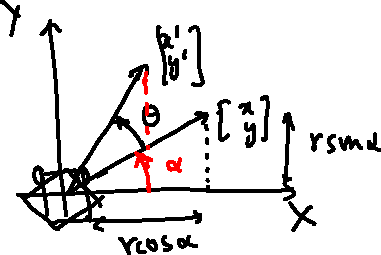
\includegraphics[width=\linewidth]{media/rotation2D-diagram.pdf}
  \caption{Rotation of points $[x, y]$ to $[x', y']$ by an angle $\alpha$}
\end{wrapfigure}
We can express original coordinates $(x,y)$ in polar coordinates,
\begin{align}
  \begin{bmatrix}
    x \\ y 
  \end{bmatrix} 
  = \begin{bmatrix}
    r \cos(\alpha) \\ r \sin(\alpha)
  \end{bmatrix} ,
\end{align}
where $r = \sqrt{x^2 + y^2}$  is the length of the vector and $\alpha  = \text{arctan2}(y, x)$ is the angle between the vector and X-axis.

The rotated points $(x', y')$ have the same length $r$ but a different angle
\begin{align}
  \begin{bmatrix}
    x' \\ y'
  \end{bmatrix} 
  = \begin{bmatrix}
    r \cos(\alpha+\alpha) \\ r \sin(\alpha + \alpha)
  \end{bmatrix} .
\end{align}
Using the trignometric identities we can write,
\begin{align}
  \begin{bmatrix}
    x' \\ y'
  \end{bmatrix} 
  = \begin{bmatrix}
    r \cos(\alpha)\cos(\alpha)-r\sin(\alpha)\sin(\alpha) \\
    r \sin(\alpha)\cos(\alpha)+r\cos(\alpha)\sin(\alpha)
  \end{bmatrix}.
\end{align}

Substituting $r\cos(\alpha) = x$ and $r\sin(\alpha) = y$, we get
\begin{align}
  \begin{bmatrix}
    x' \\ y'
  \end{bmatrix} 
  = \begin{bmatrix}
    x \cos(\alpha)-y\sin(\alpha) \\
    x \sin(\alpha)+y\cos(\alpha)
  \end{bmatrix}.
\end{align}
Writing the right hand side (RHS) as a matrix vector product,
\begin{align}
  \begin{bmatrix}
    x' \\ y'
  \end{bmatrix} 
  = \underbrace{\begin{bmatrix}
    \cos(\alpha)&-\sin(\alpha) \\
    \sin(\alpha)&+\cos(\alpha)
\end{bmatrix}}_{R}
  \begin{bmatrix}
    x \\ y
  \end{bmatrix}.
\end{align}
The matrix being multiplied here is the 2D rotation matrix.

\end{solution}

\begin{prob}
  Derive the expression for Euler angles roll $\alpha$, pitch $\beta$, yaw $\gamma$ for a given 3D rotation matrix $R = R_z(\gamma) R_y(\beta) R_x(\alpha)$.
\end{prob}
\begin{solution}


\begin{align}
  R = R_z(\gamma) R_y(\beta) R_x(\alpha)
\end{align}
\begin{align}
  \implies \begin{bmatrix}
    r_{11} & r_{12} & r_{13}  \\
    r_{21} & r_{22} & r_{23}  \\
    r_{31} & r_{32} & r_{33}  
  \end{bmatrix}
  =
  \begin{bmatrix}
    c_\gamma & -s_\gamma & 0 \\
    s_\gamma & c_\gamma & 0 \\
    0 & 0 & 1\\
  \end{bmatrix}
  \begin{bmatrix}
    c_\beta & 0 & s_\beta \\
    0 & 1 & 0\\
    -s_\beta & 0 & c_\beta \\
  \end{bmatrix}
  \begin{bmatrix}
    1 & 0 & 0\\
    0 & c_\alpha & -s_\alpha \\
    0 & s_\alpha & c_\alpha \\
  \end{bmatrix}
\end{align}
\begin{align}
  = \begin{bmatrix}
    c_\gamma & -s_\gamma & 0 \\
    s_\gamma & c_\gamma & 0 \\
    0 & 0 & 1\\
  \end{bmatrix}
  \begin{bmatrix}
    c_\beta & s_\beta s_\alpha & s_\beta c_\alpha \\
    0 & c_\alpha & -s_\alpha \\
    -s_\beta & c_\beta s_\alpha & c_\beta c_\alpha
  \end{bmatrix}
\end{align}
\begin{align}
  \implies \begin{bmatrix}
    r_{11} & r_{12} & r_{13}  \\
    r_{21} & r_{22} & r_{23}  \\
    r_{31} & r_{32} & r_{33}  
  \end{bmatrix}
  = \begin{bmatrix}
    c_\gamma c_\beta &
    c_\gamma s_\beta s_\alpha - s_\gamma c_\alpha &
    c_\gamma s_\beta c_\alpha + s_\gamma s_\alpha
    \\
    s_\gamma c_\beta &
    s_\gamma s_\beta s_\alpha + c_\gamma c_\alpha &
    s_\gamma s_\beta c_\alpha - c_\gamma s_\alpha
    \\
    -s_\beta & c_\beta s_\alpha & c_\beta c_\alpha
  \end{bmatrix}
\end{align}

\begin{align}
  \beta &= \sin^{-1}(-r_{31}) \in [-\pi/2, \pi/2]\\
  \alpha &= \text{arctan2}(r_{32}, r_{33}) \\
  \gamma &= \text{arctan2}(r_{21}, r_{11})
\end{align}

\end{solution}

\begin{prob}
  Derive the Rodrigues formula for a rotation matrix that rotates a point around a given unit vector $\bfk$ for an angle $\theta$
\end{prob}

\begin{solution}


\begin{wrapfigure}[35]{r}{0.5\linewidth}
  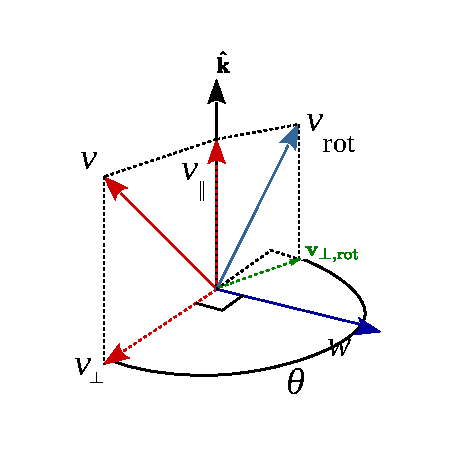
\includegraphics[width=\linewidth]{media/Rodrigues-formula.pdf}
  \caption{A vector $\bfv$ is being rotated around a unit vector $\hat{\bfk}$ by angle $\theta$. The rotated vector is called $\bfv_{rot}$. The vector $\bfv$ is split to two vectors components $\bfv_{\parallel}$ and $\bfv_\perp$. 
  Rotating $\bfv_\perp$, we obtain $\bfv_{\perp,rot}$. $\bfw$ is a vector perpendicular to both $\bfv$ and $\hat{\bfk}$. }
\end{wrapfigure}
Our strategy to derive Rodrigues formula is a three-step strategy\\
  1) Split $\bfv$ into $\bfv_\parallel$ and $\bfv_\perp$.\\
  2) Rotate $\bfv_\perp$ by angle $\theta$ to get $\bfv_{\perp,rot}$.\\
  3) Combine $\bfv_\parallel$ and $\bfv_{\perp,rot}$ to get $\bfv_{rot}$.\\

\emph{1) Split $\bfv$ into $\bfv_\parallel$ and $\bfv_\perp$}
\begin{align}
  \bfv_\parallel = (\hat{\bfk}^\top  \bfv) \hat{\bfk}
\end{align}

Find $\bfw$ such that $\bfw \perp \hat{\bfk}$ and $\bfw \perp \bfv$,
\begin{align}
  \bfw = \hat{\bfk} \times \bfv
\end{align}
Observe that the magnitude of $\bfw$ is,
\begin{align}
  |\bfw| = |\hat{\bfk} \times \bfv| = |\hat{\bfk}||\bfv|\sin(\alpha),
\end{align}
where $\alpha$ is the angle between $\hat{\bfk}$ and $\bfv$.

Find a vector $\bfu$ such that $\bfu \perp \bfw$ and $\bfu \perp  \hat{\bfk}$,
\begin{align}
  \bfu = \bfw \times \hat{\bfk} = (\hat{\bfk} \times \bfv) \times \hat{\bfk} = - \hat{\bfk} \times (\hat{\bfk} \times \bfv)
\end{align}

Note that $\bfu$ lies in the same plane as $\bfv$ and $\hat{\bfk}$ and $\bfu \perp \hat{\bfk}$. Hence, $\bfu$ is in the direction as $\bfv_\perp$. 
The magnitude of $\bfv_\perp = |\bfv|\sin(\alpha)$. The same is true for $\bfu$, $|\bfu| = |- \hat{\bfk} \times (\hat{\bfk} \times \bfv)| = |\hat{\bfk}|^2|\bfv|\sin(\alpha)\sin(90^\circ) = |\bfv|\sin(\alpha)$. Hence, 
\begin{align}
  \bfv_\perp = \bfu = - \hat{\bfk} \times (\hat{\bfk} \times \bfv)
\end{align}

\emph{2) Rotate $\bfv_\perp$ by angle $\theta$ to get $\bfv_{\perp,rot}$.}

Let $\hat{\bfu} = \frac{\bfu}{\|\bfu\|}$ be a unit-vector in the $\bfu$ direction and $\hat{\bfw} = \frac{\bfw}{\|\bfw\|}$ be a unit-vector in the $\bfw$ direction.
\begin{align}
  \bfv_{\perp,rot} &= |\bfv_\perp|\hat{\bfu} \cos(\theta) + |\bfv_\perp|\hat{\bfw} \sin(\theta)\\
                   &=\bfu \cos(\theta) + \bfw \sin(\theta).
\end{align}
The second step is true  because we know $|\bfu| = |\bfv_\perp| = |\bfw| = |\bfv| \sin(\alpha)$.
We can write $\bfv_{\perp,rot}$ in terms of cross-products,
\begin{align}
  \bfv_{\perp,rot} &=\bfu \cos(\theta) + \bfw \sin(\theta)\\
                   &= - \hat{\bfk} \times (\hat{\bfk} \times \bfv) \cos(\theta) + (\hat{\bfk} \times \bfv)\sin(\theta)
\end{align}

\emph{3) Combine $\bfv_\parallel$ and $\bfv_{\perp,rot}$ to get $\bfv_{rot}$. }

\begin{align}
  \bfv_{rot} &= \bfv_\parallel + \bfv_{\perp,rot} \\
             &= (\hat{\bfk}^\top  \bfv) \hat{\bfk} 
- \hat{\bfk} \times (\hat{\bfk} \times \bfv) \cos(\theta) + (\hat{\bfk} \times \bfv)\sin(\theta)
\end{align}

That is one-way to write Rodrigues formula but we want to express it in terms of a matrix-vector multiplication. For this we have to express, cross-product as a matrix-vector multiplication. Recall a cross-product matrix,
\begin{align}
  \hat{\bfk} \times \bfv = \underbrace{\begin{bmatrix}
    0 & -k_z & k_y\\
    k_z & 0 & -k_x\\
    -k_y & k_x & 0
\end{bmatrix}}_{[\hat{\bfk}]_\times}\bfv = [\hat{\bfk}]_\times\bfv,
\end{align}
where $\hat{\bfk} = [k_x, k_y, k_z]^\top$ and $[\hat{\bfk}]_\times$ is used to denote the cross-product matrix of vector $\hat{\bfk}$. For ease of notation, let us denote $[\hat{\bfk}]_\times$ with $K$. Thus, $\hat{\bfk} \times \bfv = K\bfv$. Now let us re-write $\bfv_{rot}$.
\begin{align}
  \bfv_{rot} &= \bfv_\parallel + \bfv_{\perp,rot} \\
             &= \bfv_\parallel - K (K \bfv) \cos(\theta) + K \bfv \sin(\theta)\\
             &= \bfv_\parallel - K^2 \bfv \cos(\theta) + K \bfv \sin(\theta).
\end{align}
To align with other terms, let's write $\bfv_\parallel = \bfv - \bfv_\perp = \bfv - (- \hat{\bfk} \times (\hat{\bfk} \times \bfv)) = \bfv + K^2 \bfv$.

\begin{align}
  \bfv_{rot} &= \bfv + K^2 \bfv - K^2 \bfv \cos(\theta) + K \bfv \sin(\theta)\\
             &= \underbrace{(I_{3\times3} + \sin(\theta)K + (1-cos(\theta)) K^2)}_{R}\bfv,
\end{align}
where $I_{3\times3}$ is an identity matrix and $R = I + \sin(\theta)K + (1-cos(\theta)) K^2$ is the desired rotation matrix.


\end{solution}

\begin{prob}
  Derive the axis-angle representation from a given 3D rotation matrix.
\end{prob}

\begin{solution}
Equate the given rotation matrix to the Rodrigues formula and solve for angle $\theta$ first,
\begin{align}
  R = I + \sin(\theta) K + (1-\cos(\theta)) K^2.
\end{align}

Compute $K^2$,
\begin{align}
  K^2 = \begin{bmatrix}
    0 & -k_z & k_y\\
    k_z & 0 & -k_x\\
    -k_y & k_x & 0
  \end{bmatrix}
  \begin{bmatrix}
    0 & -k_z & k_y\\
    k_z & 0 & -k_x\\
    -k_y & k_x & 0
  \end{bmatrix}
  = \begin{bmatrix}
    -k_z^2 - k_y^2 & k_y k_x & k_z k_x \\
    k_x k_y & -k_z^2 - k_x^2 & k_z k_y \\
    k_x k_z &  k_y k_z & -k_y^2 - k_x^2\\
  \end{bmatrix}
\end{align}

Expand the Rodrigues formula element-wise
\begin{align}
  \begin{bmatrix}
    r_{11} & r_{12} & r_{13}  \\
    r_{21} & r_{22} & r_{23}  \\
    r_{31} & r_{32} & r_{33}  
  \end{bmatrix}
  &= \begin{bmatrix}
    1 & 0 & 0\\
    0 & 1 & 0\\
    0 & 0 & 1
  \end{bmatrix}
  + \sin(\theta)
  \begin{bmatrix}
    0 & -k_z & k_y\\
    k_z & 0 & -k_x\\
    -k_y & k_x & 0
  \end{bmatrix}
  + (1-\cos(\theta))
  \begin{bmatrix}
    -k_z^2 - k_y^2 & k_y k_x & k_z k_x \\
    k_x k_y & -k_z^2 - k_x^2 & k_z k_y \\
    k_x k_z &  k_y k_z & -k_y^2 - k_x^2\\
  \end{bmatrix}\\
  &=\begin{bmatrix}
    1-(1-\cos(\theta))(k_z^2 + k_y^2), &
    - \sin(\theta) k_z + (1-\cos(\theta)) k_y k_x, &
    \sin(\theta) k_y + (1-\cos(\theta)) k_z k_x \\
    \sin(\theta) k_z + (1-\cos(\theta)) k_x k_y, &
    1-(1-\cos(\theta))(k_z^2 + k_x^2) , &
    -\sin(\theta) k_x + (1-\cos(\theta)) k_z k_y \\
    -\sin(\theta) k_y + (1-\cos(\theta)) k_x k_z, &
    \sin(\theta) k_x + (1-\cos(\theta)) k_y k_z, &
    1-(1-\cos(\theta))(k_y^2 + k_z^2)
  \end{bmatrix}
  \label{eq:rod-exp}
\end{align}

Note that the diagonal terms on the right hand side would add up to $k_x^2 + k_y^2 + k_z^2 = \|\hat{\bfk}\|^2 = 1$ which is the magnitude squared of the unit-vector $\hat{\bfk}$ which is 1.

The operation of taking the sum of diagonal elements of a matrix is called a trace operator, $\tr()$, 
\begin{align}
  \tr(R) = r_{11} + r_{22} + r_{33} = 3 - 2(1-\cos(\theta)) (k_x^2 + k_y^2 + k_z^2) = 3 - 2(1-\cos(\theta)) = 1 + 2\cos(\theta).
\end{align}
We can get $\theta$ from the above equation,
\begin{align}
  \theta = \cos^{-1}\left(\frac{\tr(R) - 1}{2}\right) \in [0, \pi].
\end{align}

Note the symmetric terms about diagonal element in Eq~\eqref{eq:rod-exp}. For example, taking the difference of $r_{21} - r_{12}$ will cancel the common term $(1-\cos(\theta)) k_x k_y$,
\begin{align}
  r_{21} - r_{12} = 2\sin(\theta)k_z \implies k_z = \frac{r_{21} - r_{12}}{2\sin(\theta)} \text{ if } \sin(\theta) \neq 0.
\end{align}

Similarly, we can find other components (when $\sin(\theta) \neq 0$),
\begin{align}
  \begin{bmatrix}
    k_x \\ k_y \\ k_z
  \end{bmatrix} 
  = \frac{1}{2\sin(\theta)}\begin{bmatrix}
    r_{32} - r_{23} \\ r_{13} - r_{31} \\ r_{21} - r_{12}
  \end{bmatrix}
\end{align}

\emph{What can we do when $\sin(\theta) = 0$? }

When $\sin(\theta) = 0$, then either $\theta = 0$ or $\theta = \pi$. If $\theta = 0$, then there is no rotation and all rotation axis are equally valid. If $\theta = \pi$ then $\cos(\theta) = \cos(\pi) = -1$. We can substitute this information in the diagonal terms and equate them. 

\begin{align}
  \begin{bmatrix}
    r_{11} & r_{12} & r_{13}  \\
    r_{21} & r_{22} & r_{23}  \\
    r_{31} & r_{32} & r_{33}  
  \end{bmatrix}
  = \begin{bmatrix}
    1-2(k_z^2 + k_y^2) & 2k_yk_x & 2k_zk_x \\
    2k_x k_y & 1-2(k_z^2 + k_x^2) & 2k_zk_y \\
    2k_xk_z & 2k_y k_z & 1-2(k_y^2 + k_x^2) \\
  \end{bmatrix}
\end{align}

For example, the first diagonal term becomes,
\begin{align}
  r_{11} = 1 - (1-(-1))(k_z^2 + k_y^2) = 1-2(k_z^2 + k_y^2).
\end{align}
Since $k_x^2 + k_y^2 + k_z^2 = 1$, then $k_z^2 + k_y^2 =  1- k_x^2$. Substitute this in above equation, to get,
\begin{align}
  r_{11} =  1-2(1-k_x^2) \implies k_x = \pm \sqrt{\frac{r_{11}+1}{2}}.
\end{align}
Similarly, $k_y$ and $k_z$ can be determined upto a sign,
\begin{align}
  \begin{bmatrix}
    k_x \\ k_y \\ k_z
  \end{bmatrix} 
  = \begin{bmatrix}
\pm \sqrt{\frac{r_{11}+1}{2}}
\\
\pm \sqrt{\frac{r_{22}+1}{2}}
\\
\pm \sqrt{\frac{r_{33}+1}{2}}
  \end{bmatrix}.
\end{align}

We know that rotation by $\pi$ around $\hat{\bfk}$ or around $-\hat{\bfk}$ is equivalent. Once we fix sign of one of the non-zero elements, say $k_x$ to be plus or minus then sign of other elements can be determined from non diagonal elements. Define a sign function,
\begin{align}
  \sign(y) = \begin{cases}
    +1 & \text{ if } y \ge 0\\
    -1 & \text{ if } y < 0
  \end{cases}.
\end{align}

Fix the sign of $k_x$ and figure out the signs of $k_y$ and $k_z$ from signs of non-diagonal terms in R.
\begin{align}
  \begin{bmatrix}
    k_x \\ k_y \\ k_z
  \end{bmatrix} 
  = \begin{bmatrix}
+ \sqrt{\frac{r_{11}+1}{2}}
\\
+\sign(r_{12}) \sqrt{\frac{r_{22}+1}{2}}
\\
+\sign(r_{13}) \sqrt{\frac{r_{33}+1}{2}}
\end{bmatrix} \text{ or  }
\begin{bmatrix}
- \sqrt{\frac{r_{11}+1}{2}}
\\
-\sign(r_{12}) \sqrt{\frac{r_{22}+1}{2}}
\\
-\sign(r_{13}) \sqrt{\frac{r_{33}+1}{2}}
\end{bmatrix}.
\end{align}
\end{solution}

\section{Homework 1}

\begin{prob}
  For the rotation matrix
  \begin{align}
  ^{XYZ}R_{UVW} = \begin{bmatrix}
    2/7 & -6/7 & 3/7\\
   6/7 & 3/7 & 2/7\\
   -3/7 & 2/7 & 6/7
  \end{bmatrix}
\end{align}
Show that $^{XYZ}R_{UVW}$ is a proper rotation matrix.
\end{prob}
\begin{solution}
A matrix $R$ is a proper rotation matrix when $R^\top R = I$ and $\det(R) = 1$. 
\begin{align}
\begin{bmatrix}
    2/7 & -6/7 & 3/7\\
   6/7 & 3/7 & 2/7\\
   -3/7 & 2/7 & 6/7
  \end{bmatrix}
\begin{bmatrix}
2/7 & -6/7 & 3/7\\
6/7 & 3/7 & 2/7\\
-3/7 & 2/7 & 6/7
\end{bmatrix}^\top = 
\begin{bmatrix}
  49/49 & 0 & 0 \\
  0 & 49/49 & 0\\
  0 & 0 & 49/49 
\end{bmatrix} \\
\det(R) = 
\det(\begin{bmatrix}
    2/7 & -6/7 & 3/7\\
   6/7 & 3/7 & 2/7\\
   -3/7 & 2/7 & 6/7
  \end{bmatrix}) = 343/343 = 1
\end{align}
\end{solution}

\begin{prob}
  For the rotation matrix
  \begin{align}
  ^{XYZ}R_{UVW} = \begin{bmatrix}
    2/7 & -6/7 & 3/7\\
   6/7 & 3/7 & 2/7\\
   -3/7 & 2/7 & 6/7\\
  \end{bmatrix}
\end{align}
Show that $R^{-1} = R^\top$.
\end{prob}
\begin{solution}

By definition of an inverse $R^{-1} R = I$ and by property of rotation matrices $R^\top R = I$, $R^{-1} = R^\top$.

\end{solution}
\begin{prob}
  For the rotation matrix
  \begin{align}
  ^{XYZ}R_{UVW} = \begin{bmatrix}
    2/7 & -6/7 & 3/7\\
   6/7 & 3/7 & 2/7\\
   -3/7 & 2/7 & 6/7
  \end{bmatrix}
\end{align}
Compute RA where matrix A is given by
\begin{align}
  A = \begin{bmatrix}
    3/7 & 2/7 & 6/7\\
    2/7 & 6/7 & -3/7\\
    -6/7 & 3/7 & 2/7
  \end{bmatrix}
\end{align}
\end{prob}
\begin{solution}
\begin{align}
  R A = \begin{bmatrix}
    2/7 & -6/7 & 3/7\\
   6/7 & 3/7 & 2/7\\
   -3/7 & 2/7 & 6/7
  \end{bmatrix} 
\begin{bmatrix}
    3/7 & 2/7 & 6/7\\
    2/7 & 6/7 & -3/7\\
    -6/7 & 3/7 & 2/7
    \end{bmatrix} 
    = \frac{1}{49}\begin{bmatrix}
-24& -23&  36\\
        12&  36&  31\\
       -41&  24& -12
  \end{bmatrix}
\end{align}

\end{solution}
\begin{prob}
  If $\bfp_{UVW} = (1, 2, 3)^\top$, what is $\bfp_{XYZ}$,
  using the rotation matrix
  \begin{align}
  ^{XYZ}R_{UVW} = \begin{bmatrix}
    2/7 & -6/7 & 3/7\\
   6/7 & 3/7 & 2/7\\
   -3/7 & 2/7 & 6/7
  \end{bmatrix}
\end{align}
\end{prob}
\begin{solution}
\begin{align}
  \bfp_{XYZ} = ^{XYZ}R_{UVW} \bfp_{UVW} = \frac{1}{7}\begin{bmatrix} -1 \\ 18 \\ 21\end{bmatrix}
\end{align}

\end{solution}
\begin{prob}
  If $\bfp_{XYZ} = (1, 2, 3)^\top$, what is $\bfp_{UVW}$,
  using the rotation matrix
  \begin{align}
  ^{XYZ}R_{UVW} = \begin{bmatrix}
    2/7 & -6/7 & 3/7\\
   6/7 & 3/7 & 2/7\\
   -3/7 & 2/7 & 6/7
  \end{bmatrix}
\end{align}
\end{prob}
\begin{solution}

\begin{align}
  \bfp_{UVW} = ^{UVW}R_{XYZ} \bfp_{XYZ} = (^{XYZ}R_{UVW})^\top \bfp_{XYZ}
  \frac{1}{7}\begin{bmatrix} 5 \\ 6 \\ 27 \end{bmatrix}
\end{align}

\end{solution}

\begin{prob}
If the OUVW system has basis vectors $\bfu = (1/\sqrt2, 0, 1/\sqrt2)^\top$, $\bfv = (-1/\sqrt2, 0, 1/\sqrt2)^\top$, $\bfw = (0, -1, 0)^\top$, and the OXYZ system has basis vectors $\bfx = (1, 0, 0)^\top$, $\bfy = (0, 1/\sqrt2, -1/\sqrt2)^\top$, $\bfz = (0, 1/\sqrt2, 1/\sqrt2)^\top$, then what is the corresponding rotation matrix between the two systems? 
\end{prob}

\begin{solution}

Recall that the columns of rotation matrix are formed by basis-vectors of the source coordinate frame represented in the destination coordinate frame.

Let the coordinates be specified in a system $OPQR$, then the rotation matrices are, 
\begin{align}
  ^{OPQR}R_{OUVW} = \begin{bmatrix}
    \bfu & \bfv & \bfw 
  \end{bmatrix} 
  = \frac{1}{\sqrt2}\begin{bmatrix} 
    1 & -1 & 0 \\
    0 & 0 & -\sqrt{2} \\
    1 & 1 & 0
  \end{bmatrix}\\
  ^{OPQR}R_{OXYZ} = \begin{bmatrix}
    \bfx & \bfy & \bfz 
  \end{bmatrix} 
  = \frac{1}{\sqrt2}\begin{bmatrix} 
    \sqrt2 & 0 & 0 \\
    0 & 1 & 1\\
    0 & -1 & 1
  \end{bmatrix}
\end{align}
A rotation matrix between the two system is,
\begin{align}
  ^{OUVW}R_{OXYZ} &= ^{OUVW}R_{OPQR} (^{OPQR}R_{OXYZ}) = (^{OPQR}R_{OUVW})^\top (^{OPQR}R_{OXYZ})\\
                  &= \frac{1}{\sqrt2}\begin{bmatrix} 
    1 & -1 & 0 \\
    0 & 0 & -\sqrt{2} \\
    1 & 1 & 0
  \end{bmatrix}^\top
  \frac{1}{\sqrt2}\begin{bmatrix} 
    \sqrt2 & 0 & 0 \\
    0 & 1 & 1\\
    0 & -1 & 1
  \end{bmatrix}\\
                  &= \frac{1}{\sqrt2}\begin{bmatrix} 
    1 & 0 & 1 \\
    -1 & 0 & 1 \\
    0 & -\sqrt2  & 0
  \end{bmatrix}
  \frac{1}{\sqrt2}\begin{bmatrix} 
    \sqrt2 & -1 & 1\\
    -\sqrt2 & -1 & 1\\
    0 & -\sqrt2 & -\sqrt2
  \end{bmatrix}\\
                  &= \frac{1}{2}\begin{bmatrix}
                    \sqrt{2} & -1 & 1 \\
                    0 & -\sqrt2 & -\sqrt2\\
                    \sqrt2 & 1 & -1
                  \end{bmatrix}
\end{align}
\end{solution}

\section{Homework 2}
We are given the following 4x4 homogeneous transformation matrices,
\begin{align}
  ^BT_A &= \frac{1}{7}\begin{bmatrix}
    2 & -6 & 3 & 7\\
    6 & 3& 2 & 14\\
    -3 & 2 & 6 & 21\\
    0 & 0 & 0 & 1
  \end{bmatrix}
        &
    ^CT_B &= \frac{1}{7}\begin{bmatrix}
    3 & 2 & 6 & 28\\
    2 & 6 & -3 & 35\\
    -6 & 3 & 2 & 42\\
    0 & 0 & 0 & 1
    \end{bmatrix}.
\end{align}
\begin{prob}
  Give the inverse of Matrix $^BT_A$
\end{prob}
\begin{solution}
\begin{align}
  \text{If }
  ^BT_A = \begin{bmatrix}
    ^BR_A & ^B\bft_A \\ 
    \mathbf{0}^\top & 1
  \end{bmatrix},
  \qquad \text{ then }
  ({}^BT_A)^{-1} = \begin{bmatrix}
    {}^BR^\top_A & - {}^BR^\top_A {}^B\bft_A \\ 
    \mathbf{0}^\top & 1
  \end{bmatrix}
\end{align}
\begin{align}
  {}^BR^\top_A &= \frac{1}{7}\begin{bmatrix}
    2 & 6 & -3 \\
    -6 & 3 & 2 \\
    3 & 2 & 6
  \end{bmatrix}\\
    - {}^BR^\top_A {}^B\bft_A &=  - \frac{1}{7}\begin{bmatrix}
    2 & 6 & -3 \\
    -6 & 3 & 2 \\
    3 & 2 & 6
    \end{bmatrix} \begin{bmatrix} 1 \\ 2 \\ 3 \end{bmatrix}
    = \frac{1}{7}\begin{bmatrix} -5 \\ -6 \\ -27 \end{bmatrix}
\end{align}

\begin{align}
  ({}^BT_A)^{-1} = \begin{bmatrix}
    {}^BR^\top_A & - {}^BR^\top_A {}^B\bft_A \\ 
    \mathbf{0}^\top & 1
  \end{bmatrix}
  = \frac{1}{7}\begin{bmatrix}
    2 & 6 & -3 & -5\\
    -6 & 3 & 2 & -6\\
    3 & 2 & 6 & -27 \\
    0 & 0 & 0 & 1
  \end{bmatrix}
\end{align}

\end{solution}
\begin{prob}
What is the direction of the X-axis of system A w.r.t. system B? What is the direction of the Y-axis of system A w.r.t system B? Where is the origin of system A w.r.t. system B?
\end{prob}
\begin{solution}
X-axis of system A in system A is $\bfx_A = (1, 0, 0)^\top$. In system B, the direction is $\bfx_B = {}^B R_A \bfx_A = (2/7, 6/7, -3/7)^\top$.


Y-axis of system A in system A is $\bfy_A = (0, 1, 0)^\top$. In system B, the direction is $\bfy_B = {}^B R_A \bfy_A = (-6/7, 3/7, 2/7)^\top$.


Origin of system A in system A is $\bfo_A = (0, 0, 0)^\top$. In system B, the origin is $\bfo_B = {}^B R_A \bfo_A + {}^B\bft_A = (1, 2, 3)^\top$.

\end{solution}
\begin{prob}
What is the direction of the X-axis of system B w.r.t. system A? What is the direction of the Y-axis of system B w.r.t system A? Where is the origin of system B w.r.t. system A?
\end{prob}
\begin{solution}

X-axis of system B in system B is $\bfx_B = (1, 0, 0)^\top$. In system A, the direction is $\bfx_A = {}^A R_B \bfx_B = (2/7, -6/7, 3/7)^\top$.


Y-axis of system B in system B is $\bfy_B = (0, 1, 0)^\top$. In system A, the direction is $\bfy_A = {}^A R_B \bfy_B = (6/7, 3/7, 2/7)^\top$.


Origin of system B in system B is $\bfo_B = (0, 0, 0)^\top$. In system A, the origin is $\bfo_A = {}^B R_A^\top \bfo_B - {}^B R_A^\top  {}^B\bft_A = (-5, -6, -27)^\top$.

\end{solution}
\begin{prob}
  What is ${}^CT_A$
\end{prob}
\begin{solution}
\begin{align}
  {}^CT_A = {}^CT_B {}^BT_A 
  &= 
  \frac{1}{7}\begin{bmatrix}
    3 & 2 & 6 & 28\\
    2 & 6 & -3 & 35\\
    -6 & 3 & 2 & 42\\
    0 & 0 & 0 & 1
    \end{bmatrix}
  \frac{1}{7}\begin{bmatrix}
    2 & -6 & 3 & 7\\
    6 & 3& 2 & 14\\
    -3 & 2 & 6 & 21\\
    0 & 0 & 0 & 1
  \end{bmatrix}
    = \frac{1}{49}\begin{bmatrix}
      0 & 0 & 0 49 & 203 \\
      49 & 0 & 0 & 70 \\
      0 & 49 & 0 & 84\\
      0 & 0 & 0 & 1
    \end{bmatrix}
    = \begin{bmatrix}
      0 & 0 & 0 1 & 29/7 \\
      1 & 0 & 0 & 10/7 \\
      0 & 1 & 0 & 12/7\\
      0 & 0 & 0 & 1
    \end{bmatrix}
\end{align}
\end{solution}
\begin{prob}
For the point $\bfp_A = (0, 1, 2)^T$ in system A, what are it's coordinates in system A?
\end{prob}
\begin{solution}
\begin{align}
  \bfp_B = {}^BR_A \bfp_A + {}^B\bft_A
  = \frac{1}{7} \begin{bmatrix}
    -6+6+7\\
    3-4+14\\
    2-12+21
  \end{bmatrix}
  = \frac{1}{7} \begin{bmatrix}
    7\\
    13\\
    11
  \end{bmatrix}
\end{align}

\end{solution}
\begin{prob}
For the point $(0, 1, 2)^T$ in system B, what are it's coordinates in system A?
\end{prob}
\begin{solution}
\begin{align}
  \bfp_A = ({}^BR_A)^\top \bfp_B - ({}^BR_A)^\top {}^B\bft_A 
  = \begin{bmatrix}
    2 & 6 & -3 \\
    -6 & 3 & 2\\
    3 & 2 & 6
  \end{bmatrix}
  \begin{bmatrix} 0 \\ 1 \\ 2 \end{bmatrix}
  +
  \begin{bmatrix} -5\\ -6\\ -27\end{bmatrix}
  = 
  \begin{bmatrix} 6-6-5\\ 3 +6-6 \\ 2+12-27 \end{bmatrix}
  = 
  \begin{bmatrix} -5\\ 3  \\ -13 \end{bmatrix}
\end{align}

\end{solution}
\section{Problem 2.6}
\begin{prob}
  For the figure shown below, find the 4x4 homogeneous transformation matrices $^{i-1}A_i$ and $^0A_i$ for $i=1,2,3,4,5$.\\
  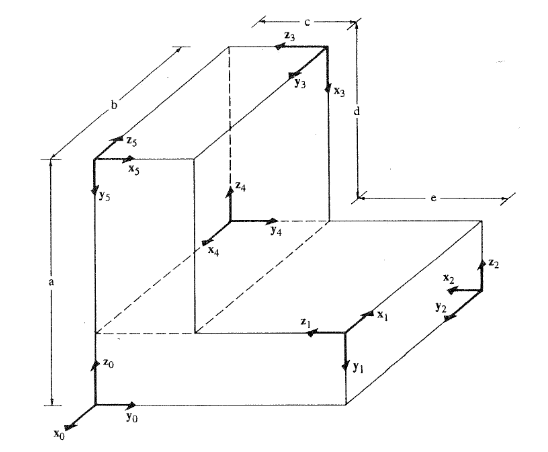
\includegraphics[width=0.5\linewidth]{media/hw3.2.6.png}
\end{prob}

\begin{solution}
Recall that the columns of rotation matrix are formed by basis-vectors of the source coordinate frame represented in the destination coordinate frame.

The translation vector is the origin of the source coordinate frame in the destination coordinate frame.

\begin{align}
  {}^0A_1 = \begin{bmatrix}
    | & | & | & | \\
    \bfx_1 & \bfy_1 & \bfz_1 & \text{Origin 1} \\
    | & | & | & | \\
    0 & 0 & 0 & 1
  \end{bmatrix}
  = \begin{bmatrix}
    -1 & 0 & 0 & 0 \\
    0 & 0 & -1 & c+e\\
    0 & -1 & 0 & a - d\\
    0 & 0 & 0 & 1
  \end{bmatrix}
  ,
\end{align}
where $\bfx_1$ is the direction of $x_1$ in terms of coordinate frame 0.

\begin{align}
  {}^0A_2 = \begin{bmatrix}
    0  & 1 &  0 & -b \\
    -1 & 0 &  0  & c+e\\
    0  & 0 &  1 & 0\\
    0  & 0 &  0 & 1
  \end{bmatrix}
  ,
  {}^0A_3 = \begin{bmatrix}
     0 & 1 &  0 & -b \\
     0 & 0 & -1  & c\\
    -1 & 0 &  0 &  a \\
     0 & 0 &  0 & 1
  \end{bmatrix}
  ,
  {}^0A_4 = \begin{bmatrix}
     1 & 0 &  0 & -b \\
     0 & 1 &  0 & 0 \\
     0 & 0 &  1 & a-d  \\
     0 & 0 &  0 & 1
  \end{bmatrix}
  ,
  {}^0A_5 = \begin{bmatrix}
     0 &  0 & -1 & 0\\
    -1 &  0 &  0 & 0\\
     0 & -1 &  0 & a\\
     0 &  0 &  0 & 1
  \end{bmatrix}
\end{align}

\begin{align}
  {}^1A_2 = \begin{bmatrix}
    0 & -1 &  0 & b \\
    0 &  0 & -1 & a-d\\
    1 &  0 &  0 & 0\\
    0 &  0 &  0 & 1
  \end{bmatrix}
  ,
  {}^2A_3 = \begin{bmatrix}
     0 & 0 &  1 & e\\
     0 & 1 &  0 & 0\\
     -1 & 0 & 0 & a\\
     0 & 0 &  0 & 1
  \end{bmatrix}
  ,
  {}^3A_4 = \begin{bmatrix}
     0 &  0 & -1 & d\\
     1 &  0 &  0 & 0\\
     0 & -1 &  0 & c\\
     0 & 0 &  0  & 1
  \end{bmatrix}
  ,
  {}^4A_5 = \begin{bmatrix}
     0 &  0 & -1 & b\\
     1 &  0 &  0 & 0\\
     0 & -1 &  0 & d\\
     0 &  0 &  0 & 1
  \end{bmatrix}
\end{align}
\end{solution}
\section{Problem 2.7}
\begin{prob}
  For the figure shown below, find the 4x4 homogeneous transformation matrices $^{i-1}A_i$ and $^0A_i$ for $i=1,2,3,4$.\\
  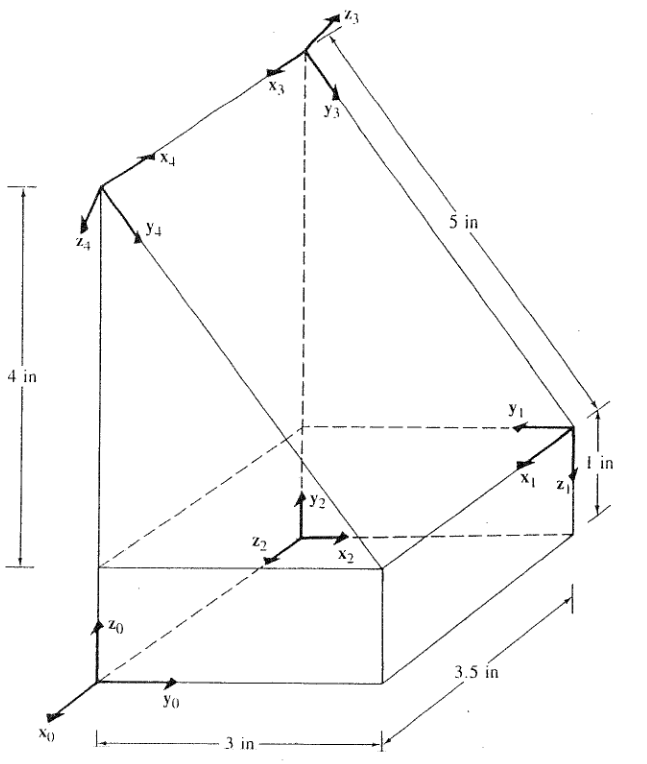
\includegraphics[width=0.5\linewidth]{media/hw3.2.7.png}
\end{prob}
\begin{solution}
Recall that the columns of rotation matrix are formed by basis-vectors of the source coordinate frame represented in the destination coordinate frame.

The translation vector is the origin of the source coordinate frame in the destination coordinate frame.

\begin{align}
  {}^0A_1 = \begin{bmatrix}
    | & | & | & | \\
    \bfx_1 & \bfy_1 & \bfz_1 & \text{Origin 1} \\
    | & | & | & | \\
    0 & 0 & 0 & 1
  \end{bmatrix}
  = \begin{bmatrix}
    1 &  0 &  0 & -3.5 \\
    0 & -1 &  0 & 3\\
    0 &  0 & -1 & 1\\
    0 & 0 & 0 & 1
  \end{bmatrix}
  ,
\end{align}
where $\bfx_1$ is the direction of $x_1$ in terms of coordinate frame 0.

\begin{align}
  {}^0A_2 = \begin{bmatrix}
    0  & 0 &  1 & -3.5\\
    1  & 0 &  0 & 0\\
    0  & 1 &  0 & 0\\
    0  & 0 &  0 & 1
  \end{bmatrix}
  ,
  {}^0A_3 = \begin{bmatrix}
     1 &    0 &    0& -3.5\\
     0 &  3/5 &  4/5& 0\\
     0 & -4/5 &  3/5& 5\\
     0 & 0 &  0     & 1
  \end{bmatrix}
  ,
  {}^0A_4 = \begin{bmatrix}
     -1 &   0  &     0 & 0\\
      0 & 3/5  &  -4/5 & 0\\
      0 & -4/5 &  -3/5 & 5\\
      0 & 0    &  0 & 1
  \end{bmatrix}
\end{align}

\begin{align}
  {}^1A_2 = \begin{bmatrix}
     0 &  0 &  1 & 0\\
    -1 &  0 &  0 & 3\\
     0 & -1 &  0 & 1\\
     0 &  0 &  0 & 1
  \end{bmatrix}
  ,
  {}^2A_3 = \begin{bmatrix}
     0 & 3/5  & 4/5& 0\\
     0 & -4/5 & 3/5& 5\\
     1 & 0    &  0 & 0\\
     0 & 0    &  0 & 1
  \end{bmatrix}
  ,
  {}^3A_4 = \begin{bmatrix}
     -1 &  0 & 0 & 3.5\\
     0 &  1 &  0 & 0\\
     0 & 0 &  -1 & 0\\
     0 & 0 &  0  & 1
  \end{bmatrix}
\end{align}
\end{solution}

\section{Labvolt Robot}
\begin{prob}
The following applies to our LabVolt robots. Draw the coordinate frame for each link (don’t forget to include link 0). Label each axis and indicate how you define the joint angles. Then fill in the joint
parameter table. Use a dot for an axis pointing out of the page and an X for an axis pointing in.\\
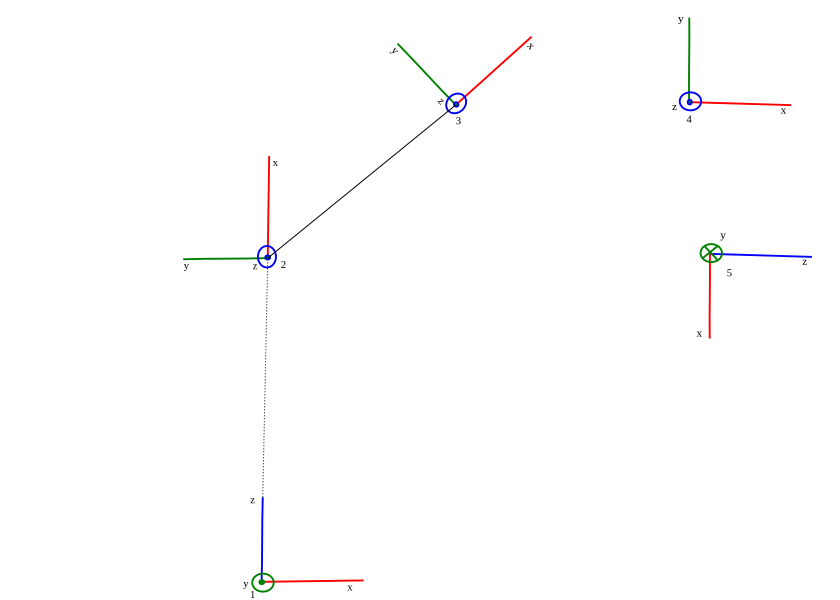
\includegraphics[width=\linewidth]{media/labvolt.png}
\end{prob}

\begin{solution}

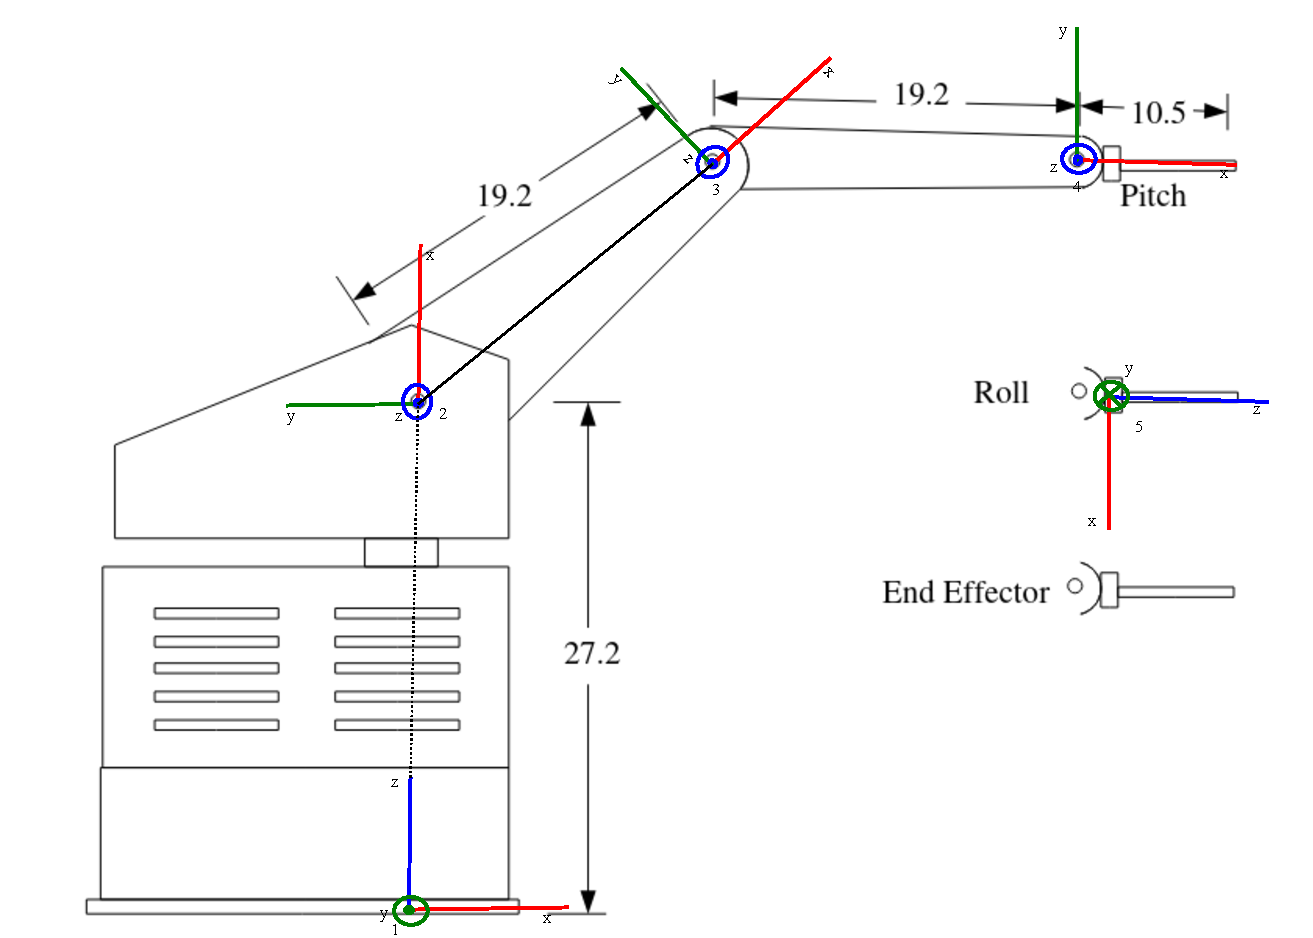
\includegraphics[width=\linewidth]{media/labvolt.png.pdf}

\begin{tabular}{rrrrr}
  \toprule
  Axis & $d_i$ & $\theta_i$ & $a_i$ & $\alpha_i$ \\
  \midrule
  1 & 27.2 & var & 0 & $90^\circ$ \\
  2 &  0.0 & var & 19.2 & 0 \\
  3 &  0.0 & var & 19.2 & 0 \\
  4 &  0.0 & var &  0.0 & $-90^\circ$ \\
  \bottomrule
\end{tabular}
\end{solution}

\end{document}

